\section{نتایج و تفسیر آن‌ها}\label{sec:results}
پس از پیاده‌سازی معماری شرح‌داده‌شده در فصل
\ref{sec:implementation}
، آزمایش کیفیت و نحوه‌ی عملکرد سامانه ضروری به نظر می‌رسد. در آزمایش‌های انجام‌شده، سامانه‌ی پیاده‌سازی شده با یکی از محبوب‌ترین نمونه‌های صنعتی، به نام \lr{Kong}، مورد مقایسه قرار گرفته شده ‌است. در ادامه، به نحوه‌ی انجام آزمایش پرداخته شده است.


\subsection{محیط آزمایش}\label{subsec:results_env}
با توجه به کاربرد وسیع درگاه‌های ارتباط با رابط‌های برنامه‌نویسی در محیط‌های ابری، انجام این آزمایش در محیط ابری به واقعیت نزدیک‌تر خواهد بود. از این رو تمام آزمایش‌ها در محیط ابری انجام شده‌است. آزمایش‌ها بر روی بستر OKD
\LTRfootnote{Openshift Kubernetes Distribution}
انجام شده‌اند.

برای ایجاد بار بر روی سامانه‌های مورد آزمایش از سکوی Locust
\cite{Locust}
استفاده شده است. میزان منابع مصرفی این سکو برای ایجاد بار به شرح زیر است:

\begin{itemize}
    \item میزان حافظه‌ی موقت مصرفی: ۱۱ گیگابایت
    \item تعداد هسته‌های پردازشی: ۲۲
    \item تعداد ایجاد‌کننده‌های بار: ۱۰
\end{itemize}

\subsection{شرح آزمایش‌ها}\label{subsec:results_tests}


\subsubsection{میزان تحمل بار}
برای بررسی میزان تحمل بار، پس از ساخت دو بطن مشابه و بدون سربار بالا، در قالب یک خدمت و استفاده از یک ضابطه‌ی مناسب به انجام آزمایش مبادرت شده است. این فرآیند در هر دو سامانه‌ی مورد ارزیابی انجام شده است.

نتایج حاصل از تولید‌ بار بر هر یک از سامانه‌ها، که در شکل‌های
\ref{highway}
و
\ref{kong}
قابل مشاهده است به شرح زیر است.

\begin{figure}[H]
    \centering
    \label{highway}
    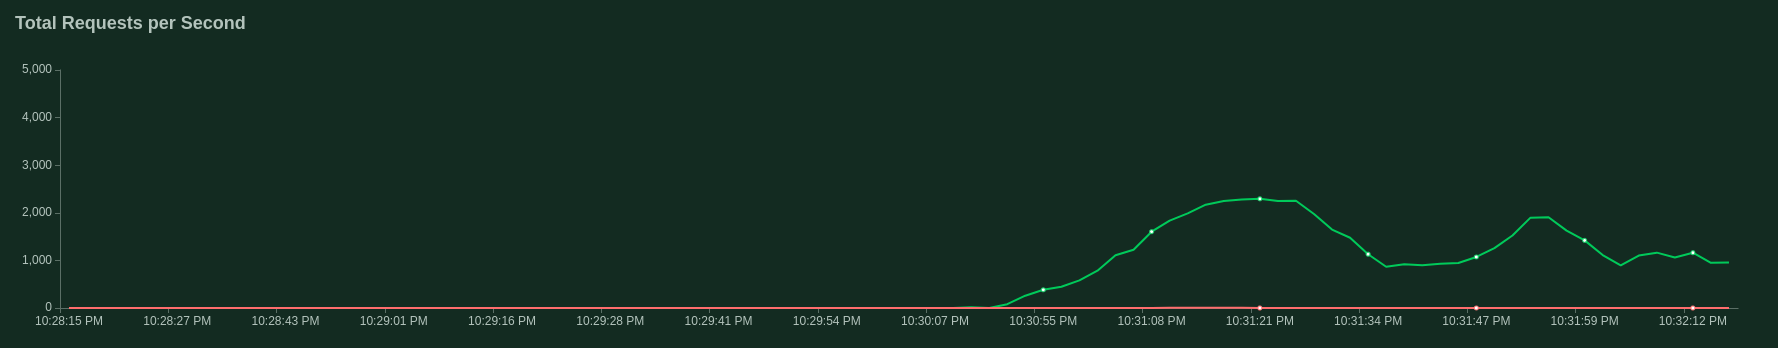
\includegraphics[scale=0.25]{images/HighwayStats.png}
    \caption{نمودار درخواست‌های سامانه‌ی پیاده‌سازی شده}
\end{figure}

\begin{figure}[H]
    \centering
    \label{kong}
    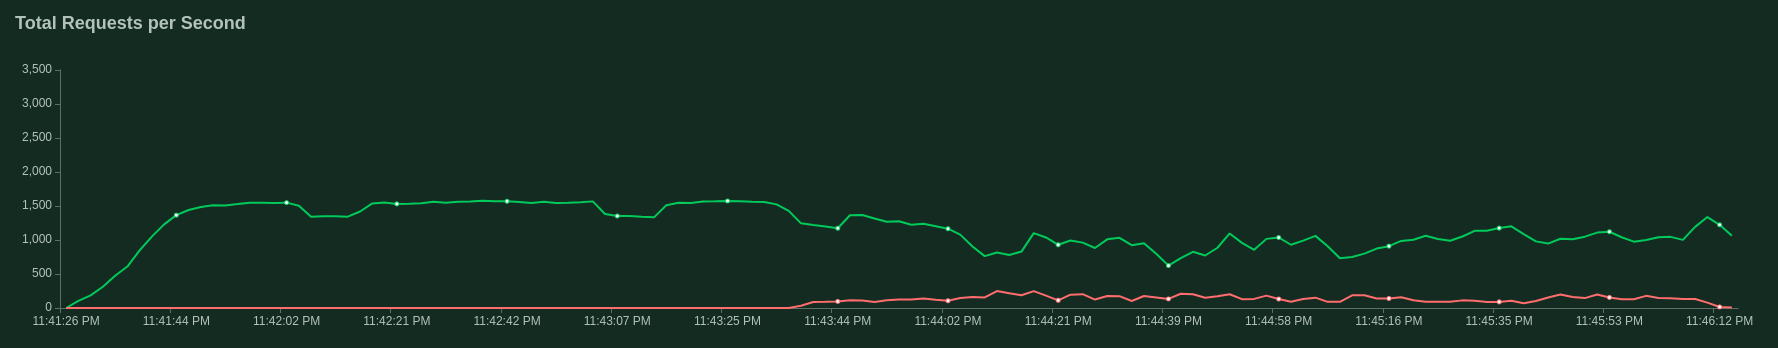
\includegraphics[scale=0.25]{images/KongStats.png}
    \caption{نمودار درخواست‌های Kong}
\end{figure}

\begin{table}[H]
    \centering
    \caption{مقایسه‌ی Kong و سامانه‌ی پیاده‌سازی شده}\label{tab:kongvshighway}
    \begin{tabular}{|c|c|c|c|}
        \hline
        محصول مورد آزمایش & بیشینه مصرف حافظه‌ی موقت & بیشینه مصرف هسته‌های پردازشی & بیشینه میزان تحمل بار\\
        \hline
        سامانه‌ی پیاده‌سازی شده & MB ۲۴۴  & ۲ & rps ۲۳۳۰ \\
        \hline
        Kong & MB ۲۰۴۸ & ۲ & rps ۱۶۴۰ \\
        \hline
    \end{tabular}
\end{table}

با توجه به جدول شماره‌ی
\ref{tab:kongvshighway}
، علی رغم کاهش ٪ ۸۸ ای میزان مصرف حافظه‌ی موقت، بیشینه میزان تحمل بار حدود ٪ ۴۲ افزایش یافته است. علاوه بر این طبق شکل شماره‌ی
\ref{highway}
، میزان درخواست‌های رد شده در سامانه‌ی پیاده‌سازی شده صفر است ولی در سامانه‌ی Kong شاهد رد شدن برخی از درخواست‌ها در اوج بار هستیم.

از این نظر، سامانه‌ی پیاده‌سازی شده بر Kong برتری کامل دارد.

\subsubsection{نحوه‌ی توزیع بار}
با توجه به وجود دو بطن برای سرویس مورد آزمایش، نحوه‌ی عملکرد توزیع‌کننده‌ی بار نیز باید مورد آزمایش قرار گیرد. با فعال کردن میان‌افزار Prometheus بر روی یک ضابطه‌ی جدید و اجرای آزمایش بر روی آن و همچنین تحلیل نتایج حاصل، می‌توان نتایج را در شکل شماره‌ی
\ref{load}
مشاهده کرد.

\begin{figure}[H]
    \centering
    \label{load}
    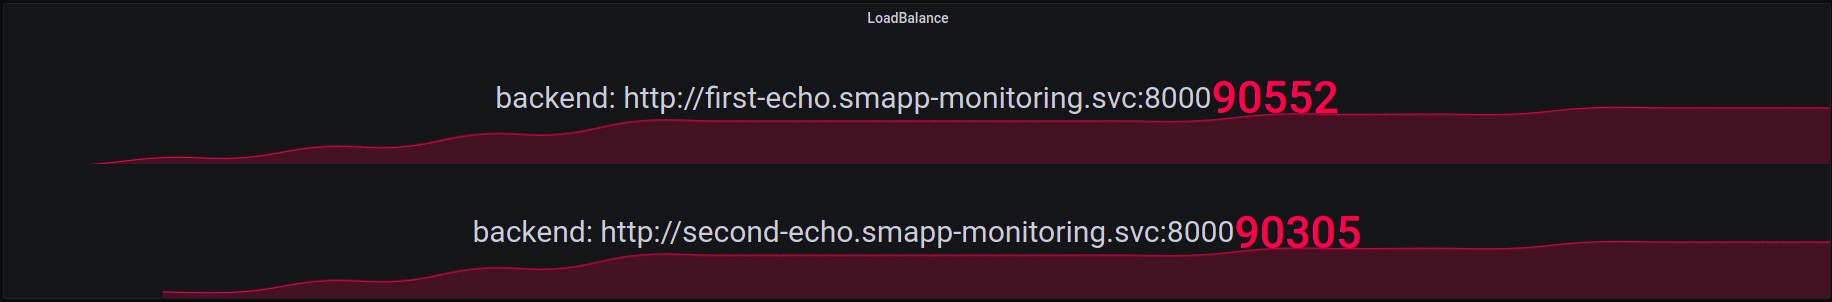
\includegraphics[scale=0.23]{images/LoadBalanceStats.png}
    \caption{نحوه‌ی عملکرد توزیع‌کننده‌ی بار}
\end{figure}

با توجه به شکل شماره‌ی
\ref{load}
، از مجموع ۱۸۰۸۷۵ درخواست ارسال شده به سامانه، ۹۰۵۵۲ به بطن اول و ۹۰۳۰۵ به بطن دوم هدایت شده اند. در مجموع ٪ ۵۰/۰۷ درخواست ها به بطن اول و ٪ ۴۹/۹۳ از درخواست‌ها به بطن دوم هدایت شده‌اند. با توجه به وزن یکسان هر دو بطن، نحوه‌ی عملکرد توزیع‌کننده بار، قابل قبول است.


\subsubsection{کنترل نرخ درخواست‌ها}
یکی از میان‌افزار‌های پیاده‌سازی شده، کنترل کننده‌ی نرخ درخواست‌ها است. برای ارزیابی این میان‌افزار و عملکرد درست آن، با ساخت یک ضابطه‌ی جدید و فعال‌سازی این میان‌افزار در آن،‌به اجرای دوباره‌ی آزمایش مبادرت شده است. نحوه‌ی پاسخ به درخواست‌ها توسط سامانه، در شکل
\ref{rate}
قابل مشاهده است.

\begin{figure}[H]
    \centering
    \label{rate}
    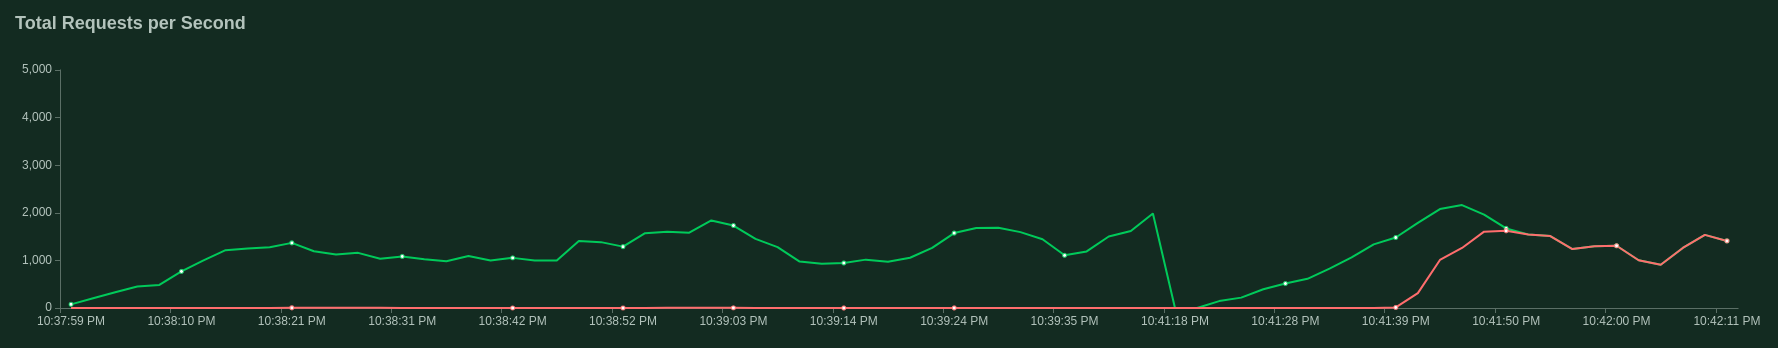
\includegraphics[scale=0.23]{images/RatelimitStats.png}
    \caption{نحوه‌ی رفتار سامانه در حضور کنترل کننده‌ی نرخ درخواست‌ها}
\end{figure}

با توجه به شکل
\ref{rate}
،‌ پس از تمام شدن تعداد درخواست مجاز هر فرستنده در زمان ۱۰:۴۱:۳۹، سامانه شروع به رد کردن درخواست‌های جدید می‌کند. از این رو، میان‌افزار پیاده‌سازی شده به درستی عمل می‌کند.

\subsubsection{رصد و تحلیل سامانه}
برای بررسی عملکرد مطلوب میان‌افزار Prometheus جهت رصد و تحلیل این سامانه، این میان‌افزار در یک ضابطه‌فعال شده و ارزیابی مجددا انجام شده است. در شکل شماره‌ی
\ref{monitoring}
، شاهد نمونه‌ی صفحه‌ی رصد سامانه هستیم. در این صفحه نحوه‌ی عملکرد توزیع‌کننده‌ی بار و همچنین Quantile های مختلف مدت زمان پاسخ‌گویی سامانه محاسبه شده است.

\begin{figure}[H]
    \centering
    \label{monitoring}
    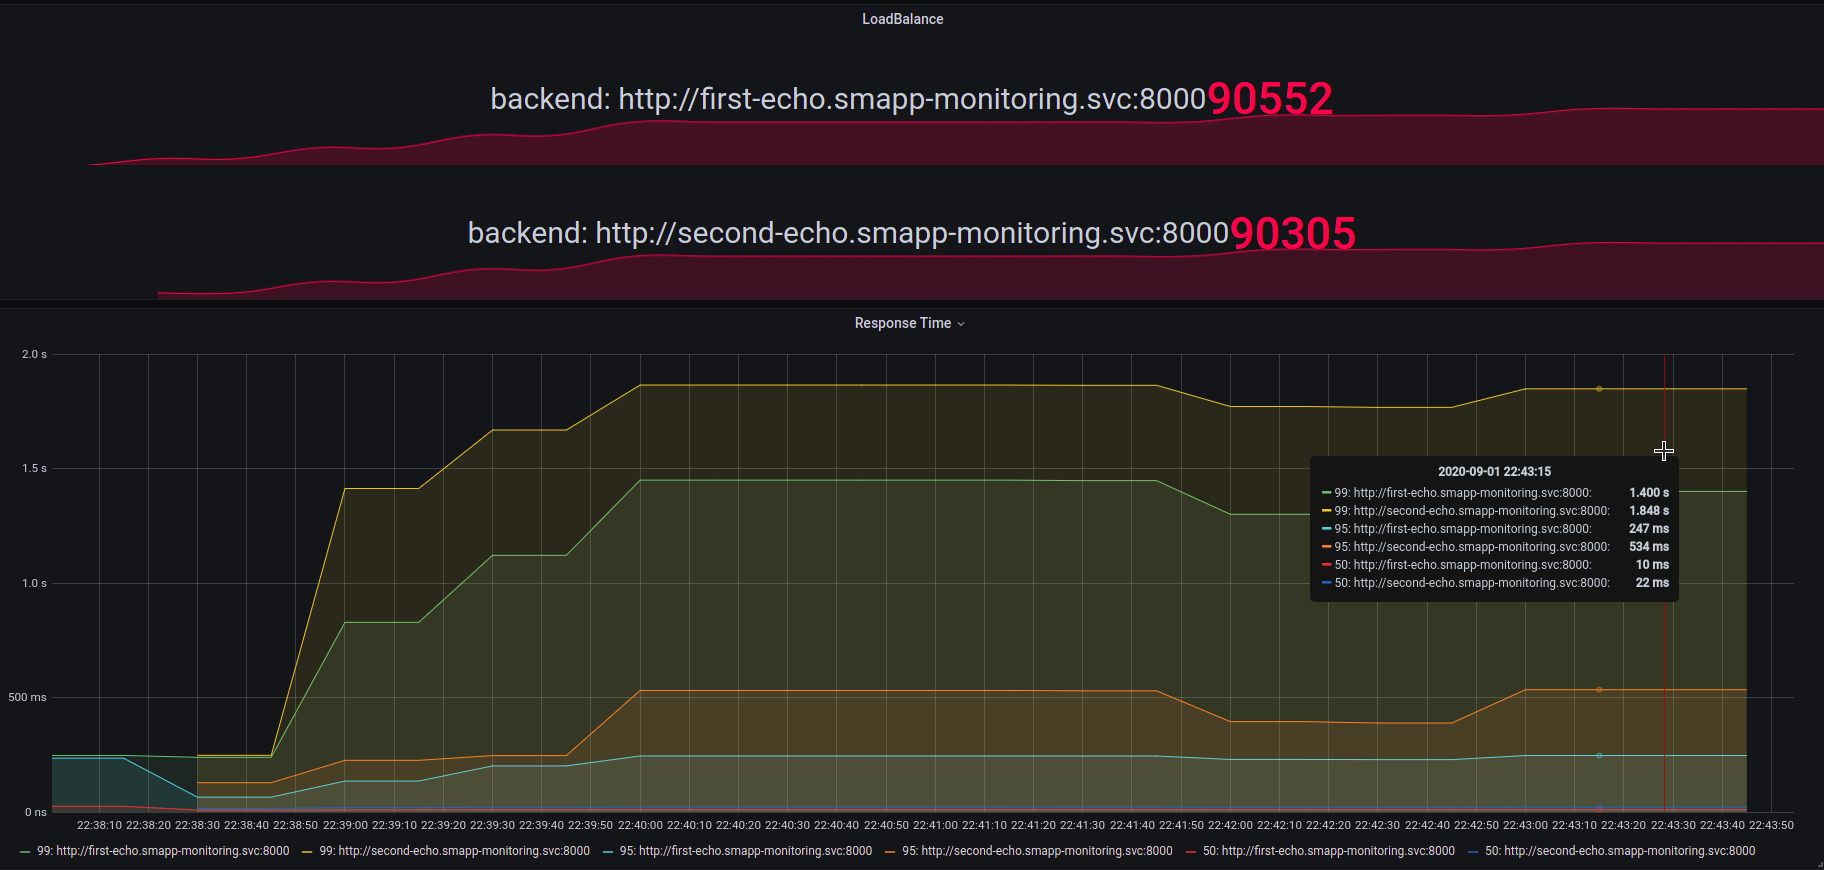
\includegraphics[scale=0.23]{images/Stats.png}
    \caption{نمونه‌ی صفحه‌ی رصد سامانه}
\end{figure}


\cleardoublepage 